%%%%%% Configurando os pacotes e comandos %%%%%%
\documentclass[fontsize=10pt]{article}
\usepackage[margin=0.70in]{geometry}
\usepackage{lipsum,mwe,abstract}
\usepackage[T1]{fontenc} 
\usepackage[brazilian]{babel} 
\usepackage{setspace}
\usepackage{caption}
\usepackage[hidelinks]{hyperref}
\usepackage{multirow}
\usepackage{booktabs}
\usepackage{float}

\usepackage{fancyhdr} % Custom headers and footers
%\pagestyle{fancyplain} % Makes all pages in the document conform to the custom headers and footers
%\fancyhead{} 
%\fancyfoot[C]{\thepage} % Page numbering for right footer
\setlength\parindent{0pt} 
\setstretch{1.5}

\usepackage{xcolor}
% Definindo novas cores
\definecolor{verde}{rgb}{0,0.5,0}
% Configurando layout para mostrar codigos C++
\usepackage{listings}
\lstset{
  language=C,
  basicstyle=\ttfamily\small,
  keywordstyle=\color{purple},
  stringstyle=\color{cyan},
  commentstyle=\color{verde},
  extendedchars=true,
  showspaces=false,
  showstringspaces=false,
  numbers=left,
  numberstyle=\tiny,
  breaklines=true,
  backgroundcolor=\color{blue!10},
  breakautoindent=true,
  captionpos=b,
  xleftmargin=0pt,
}

\usepackage{amsmath,amsfonts,amsthm} % Math packages
\usepackage{wrapfig}
\usepackage{graphicx}
\usepackage{float}
\usepackage{subcaption}
\usepackage{comment}
\usepackage{enumitem}
\usepackage{cuted}
\usepackage{sectsty} % Allows customizing section commands
\allsectionsfont{\normalfont \normalsize \scshape} % Section names in small caps and normal fonts

\renewenvironment{abstract} % Change how the abstract look to remove margins
 {\small
  \begin{center}
  \bfseries \abstractname\vspace{-.5em}\vspace{0pt}
  \end{center}
  \list{}{%
    \setlength{\leftmargin}{0mm}
    \setlength{\rightmargin}{\leftmargin}%
  }
  \item\relax}
 {\endlist}
 
\makeatletter
\renewcommand{\maketitle}{\bgroup\setlength{\parindent}{0pt}% Change how the title looks like
\begin{center}
    \textbf{
      Universidade de São Paulo\\
      Instituto de Ciências Matemáticas e Computação
    }
\end{center}
\begin{center}
  \textbf{\@title}
  \@author\\
  [3pt] 
  \@date
\end{center}\egroup
}
\makeatother
%%% Daqui pra cima é apenas configuração %%%
%%%%%%%%%%%%%%%%%%%%%%%%%%%%%%%%%%%%%%%%%%%%

%%%%%% Definindo seus dados %%%%%%

\title{\Large{Análise de algoritmos de ordenação: \\ [-6pt] Bubble Sort, Insertion Sort e Merge Sort} \\ [10pt]} 
\author{Ana Lívia Ruegger Saldanha} 
\date{\today}

%%%%%%%%%%%%%%%%%%%%%%%%%%%%%%%%%%%

%%%%%% Iniciando seu relatório %%%%%% 
\begin{document}
\maketitle


%%%%%%%%%%%%%%%%%%%%%%%%%%%%%%%%%%%%%%%%%%%%%%%%%%%%%%%%%%%
%%%                       RESUMO                        %%%
%%%%%%%%%%%%%%%%%%%%%%%%%%%%%%%%%%%%%%%%%%%%%%%%%%%%%%%%%%%
\begin{abstract}
    %%%%%% Contextualize o seu trabalho. %%%%%%%
    Este relatório apresenta uma análise teórica e experimental acerca da eficiência de três algoritmos de ordenação: bubble sort, insertion sort e merge sort. Com base na bibliografia, cada algoritmo é brevemente debatido a partir de seu funcionamento e implementação em linguagem C, identificando-se suas respectivas funções de eficiência e complexidades assintóticas (notações Big-O e Big-Omega). Essa análise é complementada com os dados obtidos experimentalmente através de medições temporais feitas também em linguagem C.
    
\end{abstract}

\rule{\linewidth}{0.5pt}

%%%%%%%%%%%%%%%%%%%%%%%%%%%%%%%%%%%%%%%%%%%%%%%%%%%%%%%%%%%
%%%                    1 INTRODUÇÃO                     %%%
%%%%%%%%%%%%%%%%%%%%%%%%%%%%%%%%%%%%%%%%%%%%%%%%%%%%%%%%%%%
\section{Introdução}
%%%%%% Faça a introdução do seu relatório. O que será feito? %%%%%%
    
    \quad O problema da ordenação apresentado por Cormen no primeiro capítulo de \textit{Algoritmos: teoria e prática} \cite{cormen} é frequentemente apresentado para introduzir o conceito de algoritmos e eficiência. Pode ser definido formalmente da seguinte maneira:
    
    \begin{itemize}
        \item \textbf{Entrada:} Uma sequência de $n$ números $<a_1, a_2, ..., a_n>$.
        \item \textbf{Saída:} Uma permutação (reordenação) $<a_1', a_2', ..., a_n'>$ da sequência de entrada, tal que $a_1' \leq a_2' \leq ... \leq a_n'$.
    \end{itemize}
    
    \quad Para solucioná-lo, podemos utilizar diversos algoritmos, mas, mesmo que todos sejam corretos e resolvam o problema dado, esses algoritmos podem ser muito diferentes em termos de eficiência. Neste relatório, temos por objetivo debater essa questão através da análise e comparação de três algoritmos de ordenação: bubble sort (ordenação por flutuação), insertion sort (ordenação por inserção) e merge sort (ordenação por intercalação). 
    
    \quad Primeiramente, buscamos contextualizar cada um dos três algoritmos abordados, apresentando seu funcionamento básico e implementações em linguagem C, assim como as funções obtidas através da contagem de operações de cada algoritmo e respectivas análises utilizando o conjunto de notações assintóticas Big-O ($\mathcal{O}$) e Big-Omega ($\Omega$).
    
    \quad Em seguida, apresentamos os resultados de um experimento realizado com os três algoritmos através de medições temporais. O experimento tem por objetivo comprovar as discussões levantadas anteriormente para que possamos, por fim, realizar uma análise abrangente desses algoritmos em diferentes cenários.


%%%%%%%%%%%%%%%%%%%%%%%%%%%%%%%%%%%%%%%%%%%%%%%%%%%%%%%%%%%
%%%           2 METODOLOGIA E DESENVOLVIMENTO           %%%
%%%%%%%%%%%%%%%%%%%%%%%%%%%%%%%%%%%%%%%%%%%%%%%%%%%%%%%%%%%
\section{Metodologia e desenvolvimento}
%%%%%% Explique a metodologia utilizada e o desenvolvimento do projeto. Como você obteve seus dados? Coloque seus códigos e embasamentos teóricos aqui se necessário. %%%%%%

\quad Abaixo, discutiremos mais a fundo cada um dos algoritmos estudados.

%%%%% 2.1 BUBBLE SORT %%%%%
\subsection{Bubble Sort}

\quad A ordenação por flutuação ou \textit{bubblesort} é um algoritmo bastante popular e, devido à sua lógica simples, de fácil implementação; porém, trata-se de uma solução ineficiente. Seu funcionamento consiste em permutar repetidamente elementos adjacentes que estão fora de ordem (flutuação de valores), ou seja, ao longo de sua execução os maiores valores vão sendo posicionados no final do vetor e os menores, no início. A seguir, apresentamos sua implementação em linguagem C.\footnote{As implementações utilizadas no experimento e reproduzidas neste relatório estão de acordo com o material apresentado em aula \cite{lab}. Já as equações e análises assintóticas apresentadas foram retiradas da bibliografia, especialmente do livro \textit{Algoritmos: teoria e prática} de Thomas Cormen \cite{cormen}.}

\begin{lstlisting}
void bubbleSort(int *vetor, int tamanho)
{
    int i, j;
    for (i = 0; i < tamanho - 1; i++)
    {
        for (j = 0; j < tamanho - 1 - i; j++)
        {
            if (vetor[j] > vetor[j + 1])
            {
                int aux = vetor[j];
                vetor[j] = vetor[j + 1];
                vetor[j + 1] = aux;
            }
        }
    }
}
\end{lstlisting}

\quad Podemos notar, pela lógica mostrada no código acima, que o algoritmo será sempre executado $n^2$ vezes, mas pode ser mais ou menos custoso a depender do número de trocas que precisarão ser realizadas. Dessa forma, para o \textit{bubblesort} o pior caso ocorre quando o vetor está inversamente ordenado, pois é quando será executado maior número de trocas; já o melhor caso ocorre quando o vetor já está ordenado e nenhuma troca precisa ser realizada.

\quad O número de operações de comparação feitas pelo \textit{bubblesort} em função do tamanho $n$ da entrada é dado por:
\begin{equation}
    \sum_{k=1}^{n-1} n - k \ \ \ \Longrightarrow \ \ \ f(n) = \frac{n^2 - n}{2}
\end{equation}

\quad Portanto, podemos afirmar que $f(n) \in \mathcal{O}(n^2)$ e $f(n) \in \Omega(n^2)$.

%%%%% 2.2 INSERTION SORT %%%%%
\subsection{Insertion Sort}

\quad O \textit{insertion sort}, ou ordenação por inserção, é um algoritmo eficiente para ordenar um número pequeno de elementos; seu funcionamento lembra a inserção ordenada de cartas em um baralho. Trata-se de um algoritmo estável (preserva a ordem de registros de chaves iguais) e adaptativo (tira vantagem da ordenação existente na entrada).

\newpage
\quad Abaixo, reproduzimos a implementação do \textit{insertion sort} em linguagem C:

\begin{lstlisting}
void insertionSort(int *vetor, int tamanho)
{
    int j;
    for (j = 1; j < tamanho; j++)
    {
        int chave = vetor[j];
        int i = j - 1;
        while (i >= 0 && vetor[i] > chave)
        {
            vetor[i + 1] = vetor[i];
            i--;
        }
        vetor[i + 1] = chave;
    }
}
\end{lstlisting}

\quad O número de operações de comparação feitas pelo \textit{insertion sort} em função do tamanho $n$ da entrada é dado, no pior caso, por:
\begin{equation}
    \sum_{k=1}^{n-1} n - k \ \ \ \Longrightarrow \ \ \ f(n) = \frac{n^2 - n}{2}
\end{equation}

\quad No melhor caso, temos:
\begin{equation}
    \sum_{k=1}^{n-1} 1 \ \ \ \Longrightarrow \ \ \ f(n) = n - 1
\end{equation}

\quad Portanto, podemos afirmar que $f(n) \in \mathcal{O}(n^2)$ e $f(n) \in \Omega(n)$.

%%%%% 2.3 MERGE SORT %%%%%
\subsection{Merge Sort}

\quad O \textit{mergesort} utiliza a lógica da divisão e conquista para executar a ordenação dos valores. É um algoritmo altamente eficiente, mesmo para entradas de grande tamanho, porém apresenta a desvantagem de necessitar de memória auxiliar.

\quad A implementação do \textit{mergesort} em linguagem C apresenta a seguinte função recursiva:

\begin{lstlisting}
void mergeSort(int *vetor, int inicio, int fim)
{
    if (fim <= inicio)
        return;

    int centro = (int)((inicio + fim) / 2.0);
    mergeSort(vetor, inicio, centro);
    mergeSort(vetor, centro + 1, fim);

    intercala(vetor, inicio, centro, fim);
}
\end{lstlisting}

\quad Ainda, é necessário o uso de uma outra função no processo de conquista: a função geralmente chamada \textit{merge} (intercala). Abaixo reproduzimos a sua implementação, também em linguagem C.

\begin{lstlisting}
void intercala(int *vetor, int inicio, int centro, int fim)
{
    int *vetorAux = (int *)malloc(sizeof(int) * (fim - inicio) + 1);

    int i = inicio;
    int j = centro + 1;
    int k = 0;

    while (i <= centro && j <= fim)
    {
        if (vetor[i] <= vetor[j])
        {
            vetorAux[k] = vetor[i];
            i++;
        }
        else
        {
            vetorAux[k] = vetor[j];
            j++;
        }
        k++;
    }

    while (i <= centro)
    {
        vetorAux[k] = vetor[i];
        i++;
        k++;
    }

    while (j <= fim)
    {
        vetorAux[k] = vetor[j];
        j++;
        k++;
    }

    for (i = inicio, k = 0; i <= fim; i++, k++)
        vetor[i] = vetorAux[k];

    free(vetorAux);
}
\end{lstlisting}

\quad Observando a implementação do \textit{mergesort}, podemos notar que seu funcionamento não depende da ordem inicial dos valores da entrada, ou seja, não há melhor ou pior caso para este algoritmo.

\quad O número de operações de comparação feitas pelo \textit{mergesort} em função do tamanho $n$ da entrada é dado por:
\begin{equation}
T(n) =
\begin{cases}
1,\ se\ n = 1
\\ 2T(\frac{n}{2}) + n,\ se\ n>1
\end{cases}
\end{equation}

\quad Para a k-ésima chamada, temos:
\begin{equation}
    T(n) = 2^k.T(\frac{n}{2^k}) + n.k
\end{equation}

\quad Chegamos, então, à forma fechada da função:
\begin{equation}
    f(n) = n.log_2n + n
\end{equation}

\quad Portanto, podemos afirmar que $f(n) \in \mathcal{O}(n\ logn)$ e $f(n) \in \Omega(n\ logn)$.



%%%%%%%%%%%%%%%%%%%%%%%%%%%%%%%%%%%%%%%%%%%%%%%%%%%%%%%%%%%
%%%                    3 RESULTADOS                     %%%
%%%%%%%%%%%%%%%%%%%%%%%%%%%%%%%%%%%%%%%%%%%%%%%%%%%%%%%%%%%
\section{Resultados}
    %%%%%% Mostre os resultados obtidos através dos cálculos. Utilize imagens se necessário. %%%%%%

\quad A seguir, apresentamos os resultados dos dois experimentos realizados a fim de estudar, na prática, a eficiência dos algoritmos apresentados no item anterior.

%%%%% 3.1 VETORES GERADOS ALEATORIAMENTE %%%%%    
\subsection{Vetores gerados aleatoriamente}

\quad O primeiro experimento realizado\footnote{Este teste foi executado no meu computador pessoal.} teve como objetivo analisar o desempenho dos algoritmos com vetores de entrada cada vez maiores. Destacamos algumas escolhas que fizemos na implementação do experimento:

\begin{itemize}
    \item Foram gerados vetores com valores aleatórios entre $0$ e $2n$, sendo $n$ o tamanho da entrada.
    
    \item Para cada tamanho de vetor, realizamos 10 iterações/medições; os valores apresentados a seguir, tanto na Tabela 1 quanto no gráfico (Figura 1), referem-se à média do tempo de execução nessas 10 iterações.
    
    \item Os testes dos três algoritmos foram realizados em uma única execução do programa, com exatamente os mesmos vetores, gerando um arquivo .csv para cada algoritmo. Os dados contidos nesses arquivos foram utilizados para plotar o gráfico reproduzido a seguir (Figura 1).
\end{itemize}

\newpage
\begin{table}[]
\centering
\begin{tabular}{@{}r|ccc@{}}
\multicolumn{1}{c|}{\multirow{2}{*}{\begin{tabular}[c]{@{}c@{}}Tamanho\\ da entrada\end{tabular}}} & \multicolumn{3}{c}{Tempo de execução médio {[}s{]}}                  \\
\multicolumn{1}{c|}{}                                                                              & \textbf{Bubble Sort} & \textbf{Insertion Sort} & \textbf{Merge Sort} \\ \midrule
25                                                                                                 & 0.000003             & 0.000002                & 0.000005            \\
100                                                                                                & 0.000038             & 0.000013                & 0.000015            \\
500                                                                                                & 0.000756             & 0.000249                & 0.000081            \\
1000                                                                                               & 0.002265             & 0.000772                & 0.000151            \\
2500                                                                                               & 0.014865             & 0.005047                & 0.000432            \\
5000                                                                                               & 0.066596             & 0.020300                & 0.000853            \\
7500                                                                                               & 0.164222             & 0.046901                & 0.001350            \\
10000                                                                                              & 0.296579             & 0.078389                & 0.001787            \\
15000                                                                                              & 0.698452             & 0.176235                & 0.002885            \\
20000                                                                                              & 1.245493             & 0.318745                & 0.003837            \\
25000                                                                                              & 2.000412             & 0.486748                & 0.004968            \\
30000                                                                                              & 2.894625             & 0.702058                & 0.005932            \\
35000                                                                                              & 3.907826             & 0.939350                & 0.006980            \\
40000                                                                                              & 5.158371             & 1.231537                & 0.007958            \\
45000                                                                                              & 6.510746             & 1.563532                & 0.009022            \\
50000                                                                                              & 8.098092             & 1.920094                & 0.010178           
\end{tabular}
\caption{Resultado das medições temporais para cada algoritmo; a média de tempo de execução foi tirada a partir de 10 iterações para cada tamanho de vetor.}
\label{Tabela 1}
\end{table}

\begin{figure}[H]
\begin{center}
    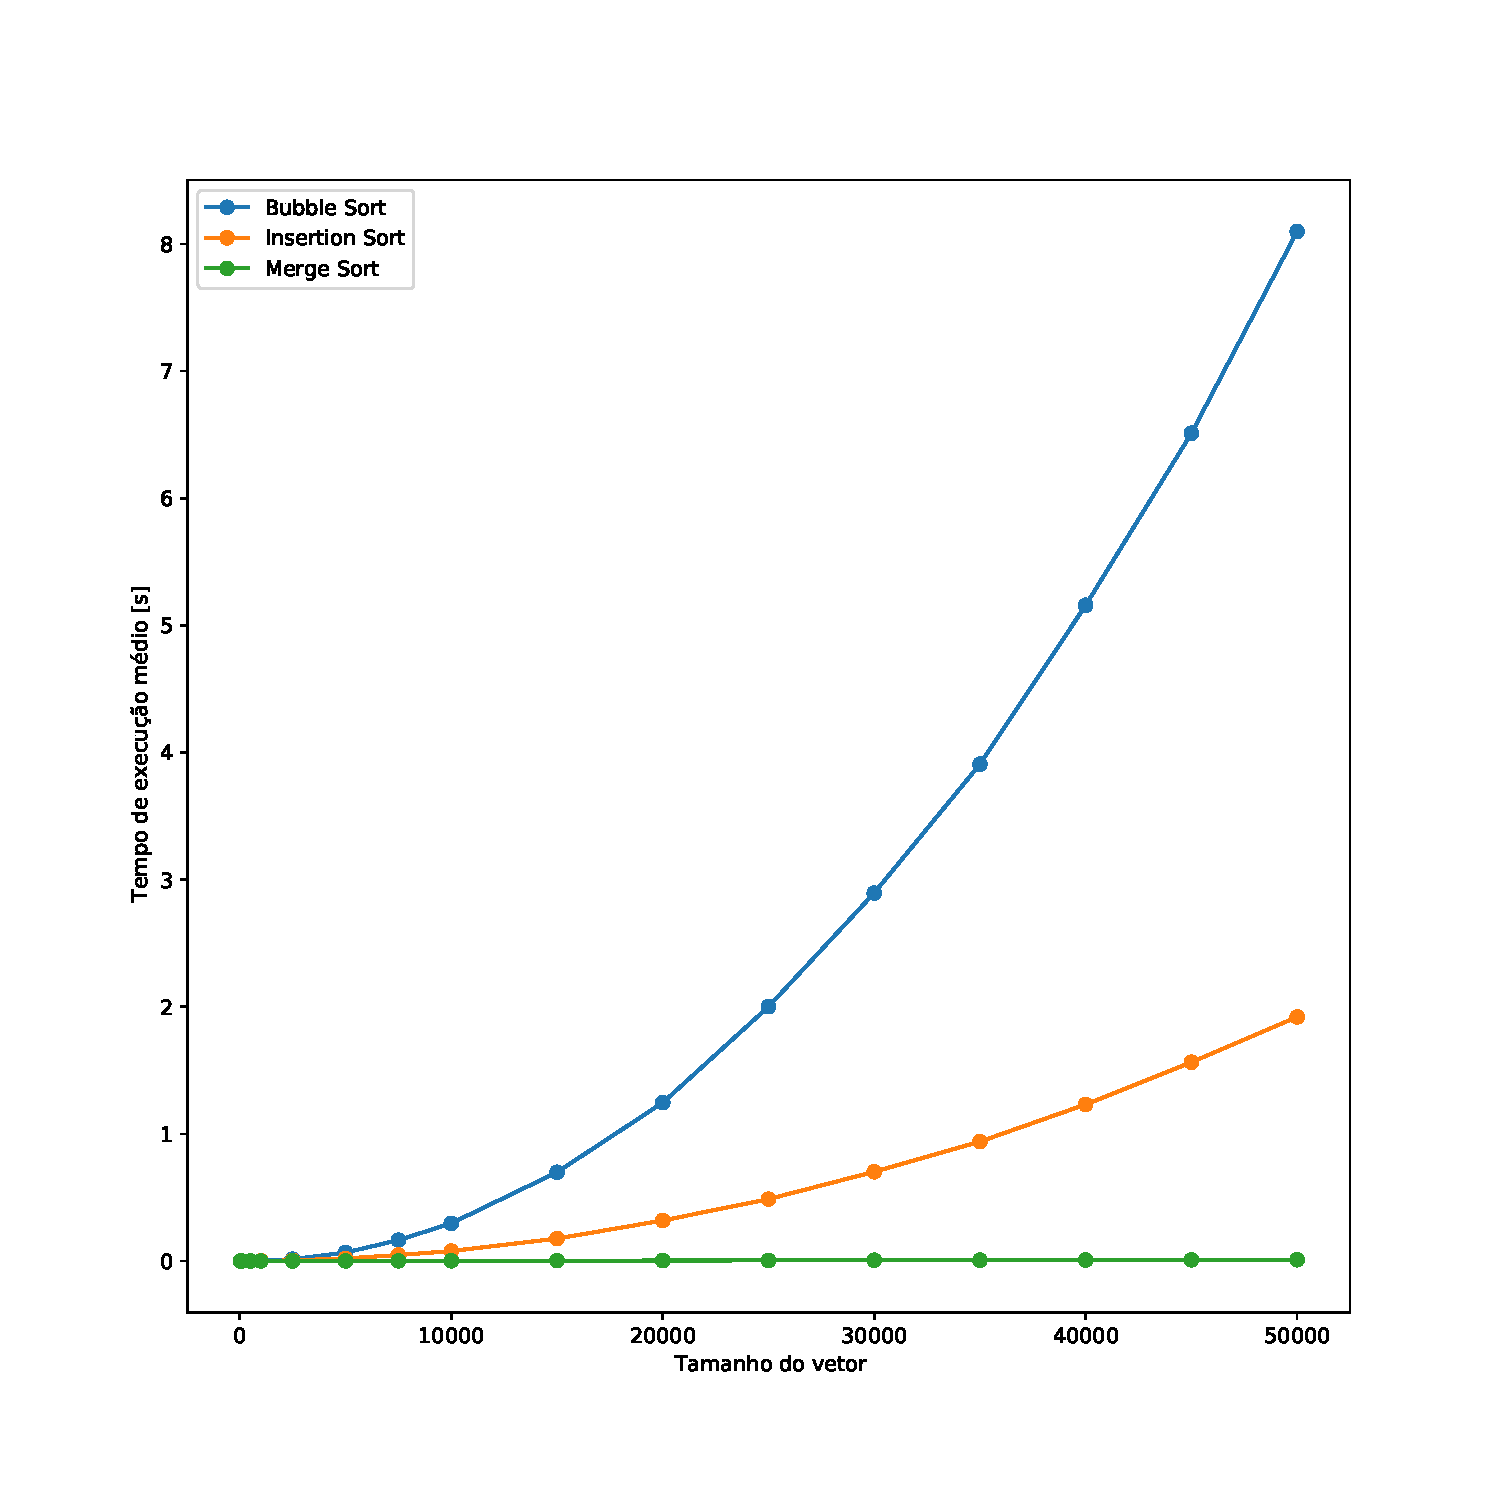
\includegraphics[scale=0.5]{comparacao.pdf}
    \caption{Resultado das medições temporais para cada algoritmo; a média de tempo de execução foi tirada a partir de 10 iterações para cada tamanho de vetor.}
    \label{Tabela 1}
\end{center}
\end{figure}

\newpage


%%%%% 3.2 MELHOR E PIOR CASO %%%%%
\subsection{Melhor e pior caso}

\quad Em um segundo experimento\footnote{Diferentemente do anterior, este teste foi realizado no GDB Online para evitar as otimizações de branch prediction do meu computador (que melhoram o significativamente o desempenho da ordenação no pior caso).}, realizamos testes com vetores de mesmo tamanho ($n = 1000$), porém de diferentes tipos: gerados aleatoriamente, ordenados e inversamente ordenados. De forma complementar ao experimento anterior, este teste visou confirmar o que foi anteriormente apontado a respeito dos melhores e piores casos para cada algoritmo.

\begin{table}[ht]
\centering
\begin{tabular}{@{}c|ccc@{}}
\multirow{2}{*}{\begin{tabular}[c]{@{}c@{}}Tipo de vetor\\ (tamanho $n = 1000$)\end{tabular}} & \multicolumn{3}{c}{Tempo de execução médio {[}s{]}}                  \\
                                                                                              & \textbf{Bubble Sort} & \textbf{Insertion Sort} & \textbf{Merge Sort} \\ \midrule
Gerado aleatoriamente                                                                         & 0.003206             & 0.000924                & 0.000182            \\
Ordenado                                                                                      & 0.001963             & 0.000006                & 0.000121            \\
Inversamente ordenado                                                                         & 0.003650             & 0.001849                & 0.000121           
\end{tabular}
\caption{Resultado das medições temporais para ordenação de diferentes tipos de vetor, todos com o mesmo tamanho; a média de tempo de execução foi tirada a partir de 10 iterações para cada tipo de vetor.}
\label{Tabela 2}
\end{table}

\quad Pelos dados apresentados na tabela acima, podemos confirmar que, de fato, o caso do vetor inversamente ordenado é o pior caso tanto para o \textit{bubblesort} quanto para o \textit{insertion sort}. Por outro lado, o vetor ordenado é o melhor caso também para ambos, ainda que, como esperado, a diferença entre o melhor e o pior caso seja muito mais expressiva no \textit{insertion sort}. No caso do \textit{mergesort}, podemos observar que não há diferença considerável entre os tempos de execução para diferentes tipos de vetor\footnote{Apesar de o caso do vetor gerado aleatoriamente ter apresentado maior tempo médio de execução, considero que os dados estejam ainda consistentes com o esperado, pois a diferença entre as médias nos três casos é muito pequena.}.

%%%%%%%%%%%%%%%%%%%%%%%%%%%%%%%%%%%%%%%%%%%%%%%%%%%%%%%%%%%
%%%                     4 CONCLUSÃO                     %%%
%%%%%%%%%%%%%%%%%%%%%%%%%%%%%%%%%%%%%%%%%%%%%%%%%%%%%%%%%%%
\section{Conclusão}
    %%%%%% Conclusão do relatório. O que você aprendeu nessa tarefa? %%%%%%
    
\quad Através dos resultados dos experimentos, pudemos confirmar as análises apresentadas no Item 2 deste relatório. Em suma:

\begin{itemize}
    \item O \textit{bubblesort} é o menos eficiente dos três algoritmos em termos de tempo de execução e número de operações executadas; quanto à memória utilizada, apresenta vantagem em relação ao \textit{mergesort} por não utilizar memória auxiliar (e iguala-se ao \textit{insertion sort} nesse aspecto).
    
    \item Em termos de tempo de execução e número de operações executadas, o \textit{insertion sort} mostrou-se melhor que o \textit{bubblesort} e pior que o \textit{mergesort}; quanto ao uso de memória, apresenta vantagem em relação ao \textit{mergesort} por não necessitar de memória auxiliar, da mesma forma que o \textit{bubblesort}. Também observa-se que este é o algoritmo mais eficiente para entradas suficientemente pequenas ($n \leq 100$).
    
    \item O \textit{mergesort} mostrou-se o mais eficiente dos três algoritmos quanto ao tempo de execução; quanto ao uso de memória, apresenta a desvantagem de necessitar de memória auxiliar.
\end{itemize}

Dessa forma, podemos concluir que, para todas as situações em que o sistema possui memória de sobra, recomenda-se o uso do \textit{mergesort}. Para os casos em que há escassez de memória, ou quando o tamanho da entrada é reduzido ($n \leq 100$), recomenda-se o uso do \textit{insertion sort}.


%%%%%%%%%%%%%%%%%%%%%%%%%%%%%%%%%%%%%%%%%%%%%%%%%%%%%%%%%%%
%%%                     REFERÊNCIAS                     %%%
%%%%%%%%%%%%%%%%%%%%%%%%%%%%%%%%%%%%%%%%%%%%%%%%%%%%%%%%%%%
\nocite{*}
\bibliographystyle{plain}
\bibliography{references.bib}
    %%%%%% Lembre-se de adicionar as referências bibliográficas utilizadas no arquivo 'references.bib'e depois cita-las nessa seção. Conulta: https://pt.overleaf.com/learn/latex/Bibliography_management_in_LaTeX %%%%%%

\end{document}